\documentclass[12pt, a4paper]{article}
\usepackage[utf8]{inputenc}
\usepackage{bookmark}
\usepackage[margin=1in]{geometry} 
\usepackage{amsmath,amsthm,amssymb}
\usepackage[margin=1in]{geometry} 
\usepackage{amsmath,amsthm,amssymb}
\usepackage{multicol}
\usepackage[slovene]{babel}
\usepackage{color}
\usepackage{graphicx}
\usepackage{amssymb}
\usepackage{amsmath}
\usepackage{mathtools}
\usepackage{commath}
\usepackage{ragged2e}
\usepackage[T1]{fontenc}
\usepackage[normalem]{ulem}
\usepackage{amsthm}
\usepackage{esvect}
\usepackage{float}
\usepackage{calrsfs}
\usepackage{tocloft}
\DeclareMathAlphabet{\pazocal}{OMS}{zplm}{m}{n}
\newcommand{\Ga}{\mathcal{G}}

\title{Rimska cesta}
\author{Matic Tonin, Gregor Humar, Rok Kuk}
\date{May 2020}

\begin{document}

\begin{center}
\thispagestyle{empty}
\parskip=14pt%
\vspace*{3\parskip}%
\begin{Huge}Rimska cesta \end{Huge}


Projekt v sklopu predmeta \\
Astronomija 1

Avtorji:

Matic Tonin, Gregor Humar, Rok Kuk

Mentor 

(Profesor: Tomaž Zwitter,Asistentka: Dunja Fabjan)

\rule{7cm}{0.4pt}

Pod okvirom:

FAKULTETE ZA FIZIKO IN MATEMATIKO, LJUBLJANA

Akademsko leto 2019/2020

\end{center}
\pagebreak
\section{Povzetek}

Ga napišemo po izvedbi vsega.

\pagebreak
\section{Uvod}

Vesolje, kot ga danes spoznavamo, je sestavljeno iz barionske snovi, temne snovi in temne energije. Pod barionsko snov pa se štejejo tudi galaksije. V vesolju je okoli 200 miljard galaksij s starostjo približno 13.8 miljard let \cite{stevilo} in ena izmed teh galaksij je tudi naša galaksija-Rimska cesta. \\
Rimska cesta ali Mlečna cesta je spiralna galaksija, po Hubblovi klasifikaciji galaksija tipa Sbc, sestavljena iz dveh glavnih krakov, Scutum-Centaurus in Perseus \cite{kraki} in prečke, ki se nahaja v središču Galaksije. Poleg krakov in prečke pa Rimsko cesto sestavljajo disk velikosti 37 kpc in debeline  približno 1 kpc \cite{dimenzije}, temni halo, ki mu je težko določiti velikost saj ni veliko zvezd v njem (120kpc)\cite{dimenzije}, temna snov, ki predstavlja velik delež mase Gakalsije ($10^{12} M_\odot$), medzvezdni prah, ki je 10 \% mase vseh zvezd \cite{prah} in super masivna črna luknja, ki se nahaja v središču Galaksije. \\
V krakih Galaksije pa lahko najdemo več kot 250 miljard zvezd, s skupno maso približno $4.6 \cdot 10^{10} M_\odot$, najdemo pa jih tudi v zvezdnem haloju, kjer so zvezde povezane med seboj v krogelna območja in zvezdne kopice ($10^{4}-10^{6}$ zvezd sestavljenih v kopico, ki ima premera od 10-50 pc).

\begin{figure}[H]
    \centering
    \includegraphics[width=10cm, height=7cm]{Rimska cesta.jpg}
    \label{fig:rimska}
    \caption{Slika Rimske ceste s ptičje perspektive, kjer se lepo vidita dva glavna kraka in sredinska prečka, Vir \cite{galaksija}}
\end{figure}
Na nočnem nebu pa jo z Zemlje vidimo kot megličast pas bele svetlobe, saj se nahajamo znotraj Rimske ceste. Naša oddaljenost od središča je okoli 8 kpc\cite{oddaljenost}, okoli njega pa se vrtimo s hitrostjo približno 220 $\frac{km}{s}$. Sklepali bi, da se glede na razdaljo od središča hitrost vrtenja zvezd manjšala, a se v resnici ohranja, kar nam da vedeti, da se ne nahaja vsa masa v središču Rimske ceste, ampak je prerazporejena po območju Galaksije. Glede na število zvezd v naši galaksiji pa bi sklepali, da je v okolici našega osončja vsaj kakšna druga zvezda. Po kratkem izračunu pa ugotovimo, da je lokalna gostota zvezd okrog nas v radiju 1pc enaka $7.3-10 \cdot 10^{-21}\frac{kg}{m^3}$ in od tega je kar $1.7 \cdot 10^{-21}\frac{kg}{m^3}$ medzvezdne snovi.\cite{opticna} \\
Pri opazovanju predmetov znotraj naše galaksije pa se bo ta medzvezdna snov poznala, prišlo bo do ekstinkcije. Ta beseda opisuje pojav, ko se elektromagnetno valovanje (fotoni) pri potovanju od opazovanega objekta do nas, absorbirajo in izgubijo v prašnih delcih. Prvič jo je v svojih delih omenjal Robert Julius Trumpler, ki je pri opazovanju zvezdnatih kopic ugotovil, da bolj kot so oddaljene, večje so, kar pa ni povsem logično, saj bi morale biti iste velikosti. Zato je sklepal, da se je svetloba pri potovanju do nas izgubila v neki snovi, ni pa vedel točno, za katero snov gre. Kasneje so ugotovili, da je ta snov plin in da zaradi tega pojava dobimo drugačen emisijski spekter, kot bi ga morali dobiti v resnici. Takemu pojavu pravimo tudi pordečitev. Razlog pa se skriva v tem, da prah absorbira ali odbije valovne manjše valovne dolžine modrega in vijoličnega spektra, saj je njihova valovna dolžina krajša in lažje reagirajo s prašnimi delci. Za daljše svetlobe pa prah zgolj zmanjša njihovo intenziteto, da na koncu dobimo, da se predmet zaradi prehajanja svetlobe skozi snov, pordeči \cite{pordecitev}.
\begin{figure}[H]
    \centering
    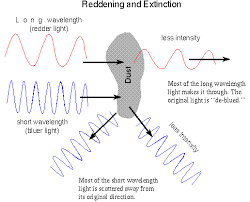
\includegraphics[width=12cm, height=9cm]{ex1.png}
    \label{fig:pordecitev}
    \caption{Postopek absorbcije in odboja svetlobe pri prehodu skosi prah, Vir \cite{pordecitev}}
\end{figure}
Da pa lahko opazimo ta pojav pa v resnici ne potrebujemo opazovati galaksije ali zvezd, saj ga lahko vsak večer srečamo na našem nebu. Iz istega razloga, se tudi Sonce, ko se bliža večer, začne obarvati oranžno in nebo se obarva rdeče, saj prihaja je pot svetlobe daljša in tako pojav pride bolj do izraza kot podnevi\cite{ekstinkcija2}.\\


Za primer B,V spektra lahko tako definiramo, da je vrednost presežka pordečitve kar enaka:

$$E_{B-V}=(B-V)_{ekstinkcije}-(B-V)_{intrinzični}$$

kjer je $(B-V)_{ekstinkcije}$ zaznana svetloba, ki jo dobimo pri opazovanju, $(B-V)_{intrinzični}$ pa dejanska vrednost, ki bi jo morali dobiti. Torej je barva galaksije, ki jo vidimo, v resnici drugačna, kot pa je dejanska in je odvisna od količine snovi, ki se nahaja med nami in opazovanim delom naše galaksije. Za zvezde, ki se nahajajo v galaktičnem disku in so nam relativno blizu (1 kpc), se nam magnituda zvezd spremeni za 1.8 $\frac{magnitudes}{kpc}$.\cite{pordecitev} \\


Ampak ta vrednost se glede na območja, kjer merimo spreminja. Zato moramo paziti, katero območje si izberemo, za merjenje naše razdalje, saj je prah po galaksiji razdeljen različno.

Če si pogledamo, kako je prerazporejen prah glede na komponente galaksije:
\begin{enumerate}
    \item \texttt{Galaktični disk:}\\
    Galaktični disk vsebuje veliko količino galaktičnega prahu, saj je galaksija spiralna in je tako veliko nastanka novih zvezd. 
    \item \texttt{Galaktični halo:}\\
    Kakor vidimo na sliki \ref{fig:Galaxydust}, je v galaktičnem haloju bolj malo prahu, saj se zaradi gravitacije, ga največ nabere v disku. 
    \item \texttt{Galaktična prečka:}\\
    V galaktični prečki se snov nabira in kroži okoli super masivne črne luknje v sredini. 
\end{enumerate}

\begin{figure}[H]
    \centering
    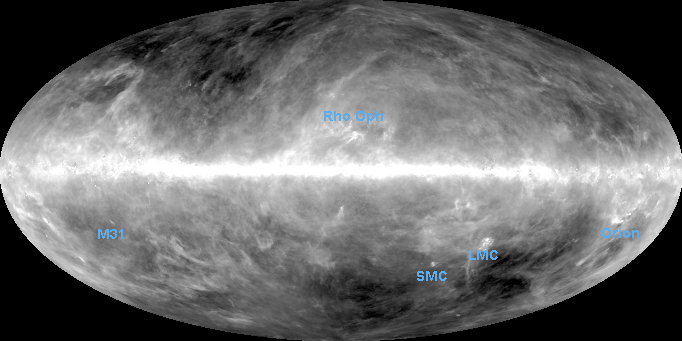
\includegraphics[width=15cm, height=9cm]{Prah.jpg}
    \label{fig:Galaxydust}
    \caption{Porazdelitev prahu v naši galaksiji, Vir \cite{Galaxydust}}
\end{figure}
Hkrati pa je mogoče tudi dokazati, kar bomo dokazali v rezultatih, da je absorbcija odvisna tudi od razdalje potovanja skozi snov. To se nam v resnici zdi logično, saj če svetloba prepotuje večjo pot, bo prepotovala skozi več snovi in bo tako naš efekt pordečitve močnejši. Kasneje bomo dokazali (z nekaj predpostavkami), da izsev zvezde, ki ga zaznamo, eksopnentno pada z optično globino, razdaljo med nami in predmetom.\cite{opticna}

\begin{equation} \label{eq:Eq1}
	   L=L_{\odot}e^{-\tau}
		\end{equation}
Kjer je $\tau$ optična globina, $L_{\odot}$ pa Sončev izsev.


\pagebreak
\section{Rezultati}
\subsection{Izpeljava formul za merjenje optične globine}
Splošno vemo, da se zakon za  magnitude glasi:
\begin{equation} \label{eq:Eq2}
	   m-m_{\odot}=-2.5\log\left(\frac{j(r)}{j_{\odot}}\right)
		\end{equation}
In enačbo za absolutne magnitude:
\begin{equation} \label{eq:Eq3}
	   m-M=5\log\left(\frac{r}{10pc}\right)
		\end{equation}
Kjer je m navadna magnituda, M pa absolutna magnituda, r pa razdalja med nami in predmetom. Kot smo zapisali, nam ekstinkcija spremeni magnitudo za nek faktor A. To lahko zapišemo z naslednjo zvezo:
\begin{equation} \label{eq:Eq4}
	   m-M=5\log\left(\frac{r}{10pc}\right)+A
		\end{equation}
Sedaj potrebujemo le še izpeljati, kolikšna je konstanta A.\\

Kot smo predpostavili v navodilih, vse zvezde izsevajo Sončev izsev $L_{\odot}$, nas pa zanima, koliko se je izgubi, ko pride skozi plast dr. Vidimo, da ko gre izsev $L$ skozi plast $dr$, se izgubi za nek faktor $\alpha$. Enačba se tako glasi:
$$dL=-\alpha L dr$$
$\alpha$ nam v resnici pove, kako učinkovita je snov pri odstranjevanju svetlobe, ko ta potuje proti nam. Če definiramo, da je optična globina, torej globina, ki jo lahko dosežemo, preden se svetlobni tok popolnoma razporedi enaka:
$$d\tau=\alpha dr$$
Tako sledi, da je v resnici moč, ki se ohranja enaka kar:
$$\int_{L_{odot}}^{L}\frac{dL}{L}=-\int_{0}^{\tau}d\tau$$
Po integraciji, dobimo izraz, s katerim lahko iz izseva izvemo, kolikšna je globinska ostrina:
\begin{equation} \label{eq:Eq5}
	  \underline{\tau=\ln\left(\frac{L_{\odot}}{L}\right)}
		\end{equation}
\medskip
Če pa naprej izrazimo izsev s svetlobnim tokom z enačbo $L=\omega r^2 j(r)$ in $L_{\odot}=\omega R^2 j_{\odot}$, kjer je $\omega$ površinski kot, $r$ je razdalja med nami in zvezdo, $R$ je radij zvezde, dobimo, da je:
\begin{equation} \label{eq:Eq6}
	  j(r)=j_{\odot}\frac{R^2}{r^2}\cdot e^{-\tau}
		\end{equation}
\medskip

Iz enačb za magnitude (\ref{eq:Eq2}) lahko sedaj vstavimo našo izpeljano zvezo za $\frac{j(r)}{j_{\odot}}$ (\ref{eq:Eq6}), dobimo:

$$m-m_\odot =-2.5 \log\left(\frac{r^2}{R^2}e^{-\tau}\right)$$

Če sedaj spremenimo to v absolutne magnitude, dobimo enačbo:
\begin{equation} \label{eq:Eq7}
	  m-M_\odot =5 \log\left(\frac{r^2}{10 pc}\right)-2.5 \log\left(e^{-\tau}\right)
		\end{equation}
		
S primerjavo enačbe (\ref{eq:Eq7}) in enačbe (\ref{eq:Eq4}) pa kmalu ugotovimo, da je:

\begin{equation} \label{eq:Eq8}
	 \underline{A=-2.5 \log\left(e^{-\tau}\right)}
\end{equation}

In tako smo izpeljali enačbo za modul razdalje s popravkom.

\medskip
\subsection{Pogled na teleskop}
Opazovali bomo s teleskopom Vega, ki ima 3 različna gorišča, eno primarno in dva sekundarna, dodatne opise navedemo kasneje. Najprej pa bomo videli, koliko zvezd zajamemo na našo sliko. \\
\medskip

Če definiramo kotno velikost slike kot $\theta$, ki je prostorski kot, ki ga zajamemo. Za teleskop imamo podano vrednost, povečave, koliko kotnih stopinj zajamemo na posamezen piksel kamere, kar bomo zapisali s količino $B$. Za kamero pa imamo podano, koliko pikslov ima določena slika in to bomo zapisalo s črko $x$. Če sedaj pogledamo, kolikšen prostorski kot zajame naš teleskop. Z danimi podatki, lahko zapišemo:
\begin{equation} \label{eq:Eq9}
	 \theta=B \cdot x \frac{\pi}{180}
	 \end{equation}
Kot $\theta$, ki ga dobimo je podan v ° zato moramo to pretvoriti v radiane. zato smo dodali faktor $\frac{\pi}{180}$. Da pa bi videli, koliko pc zajamemo v našo sliko, moramo zapisati odvisnost kota od velikosti slike. Če bi si narisali, bi kmalu ugotovili, da dobimo odvisnost oddaljenosti od velikosti slike z funkcijo tangens, da velja $\tan(\theta)=\frac{D}{r}$, kjer je D velikost polmera predmeta, r pa razdalja do predmeta. Če tangens razvijemo za majhne kote in vstavimo odvisnost za $\theta$ iz enačbe (\ref{eq:Eq9}), dobimo
\begin{equation} \label{eq:Eq10}
	 D= r \cdot B \cdot x \frac{\pi}{180}
	 \end{equation}
\pagebreak
Za primer, da bomo videli, kako veliko sliko zajamemo v x in y smeri vzemimo primer 1 kpc. To sedaj vstavimo v vse filtre:


\pagebreak
%Kazalo 
\tableofcontents

\pagebreak
%Kazalo slik
\listoffigures

\pagebreak
%Kazalo virov
\begin{thebibliography}{9}
\bibitem{stevilo}
Elizabeth Howell: How Many Galaxies Are There?, March 30, 2018 \\
\texttt{https://www.space.com/25303-how-many-galaxies-are-in-the-universe.html}

\bibitem{kraki}
Caltech/R. Hurt: The Milky Way Galaxy, November 8, 2017 \\
\texttt{https://solarsystem.nasa.gov/resources/285/the-milky-way-galaxy/}

\bibitem{dimenzije}
Croswell, Ken: Astronomers have found the edge of the Milky Way at last March 23, 2020 \\
https://www.sciencenews.org/article/astronomers-have-found-edge-milky-way-size

\bibitem{prah}
\texttt{$https://en.wikipedia.org/wiki/Milky_Way$}

\bibitem{oddaljenost}
Phil Newman: The Milky Way, May 7, 2018 \\
\texttt{$https://imagine.gsfc.nasa.gov/features/cosmic/milkyway_info.html$}

\bibitem{ekstinkcija}
Whittet, Douglas C. B.: Dust in the Galactic Environment, 2003 \\
\texttt{$https://books.google.com/books?id=k21lk4sORpEC\&pg=PA10$}

\bibitem{galaksija}
Slika \ref{fig:rimska}: \\
\texttt{$https://solarsystem.nasa.gov/internal_resources/125/$}

\bibitem{pordecitev}
Slika \ref{fig:pordecitev}: \\
Avtor neznan: Colour and Interstellar Clouds 20. june 2002 \\
\texttt{$http://www.chm.bris.ac.uk/webprojects2002/murphy/colour_and_interstellar_clouds.htm$}

\bibitem{Galaxydust}
Slika \ref{fig:Galaxydust}: \\
Schlegel, Finkbeiner in Davis, 1998 \\
\texttt{$https://irsa.ipac.caltech.edu/applications/DUST/dustbw_ann.jpg$}
\end{thebibliography}
\end{document}